%
% $RCSfile: component_oriented_programming.tex,v $
%
% Copyright (C) 2002-2008. Christian Heller.
%
% Permission is granted to copy, distribute and/or modify this document
% under the terms of the GNU Free Documentation License, Version 1.1 or
% any later version published by the Free Software Foundation; with no
% Invariant Sections, with no Front-Cover Texts and with no Back-Cover
% Texts. A copy of the license is included in the section entitled
% "GNU Free Documentation License".
%
% http://www.cybop.net
% - Cybernetics Oriented Programming -
%
% http://www.resmedicinae.org
% - Information in Medicine -
%
% Version: $Revision: 1.1 $ $Date: 2008-08-19 20:41:06 $ $Author: christian $
% Authors: Christian Heller <christian.heller@tuxtax.de>
%

\section{Component Oriented Programming}
\label{component_oriented_programming_heading}
\index{Component Oriented Programming}
\index{COP}
\index{Component Based Design}
\index{CBD}
\index{Software Component}
\index{Component}
\index{Black Box Reuse}
\index{Graphical User Interface}
\index{GUI}
\index{Delphi}
\index{Visual Component Library}
\index{VCL}
\index{Visual Basic}
\index{VB}
\index{Java}
\index{Abstract Window Toolkit}
\index{AWT}
\index{Bean}
\index{Agent}
\index{Open Source Software}
\index{OSS}
\index{Legacy System}
\index{PL/1}
\index{Interface Definition Language}
\index{IDL}
\index{Common Object Request Broker Architecture}
\index{CORBA}
\index{Aspect Oriented Programming}
\index{AOP}
\index{Aspect}
\index{Concern}
\index{Agent Oriented Programming}
\index{AGOP}
\index{Agent}

In the not-so-distant past, there has been a lot of buzz in the industry
touting \emph{Component Based Design} (CBD). Much of it was more marketing than
the actual application of new design principles and it is also no surprise that
the definition of a \emph{Software Component} differs between authors, companies
and projects. A rather formal one is that of the \emph{Avalon} framework
\cite{avalon} of the \emph{Apache Jakarta} project \cite{jakarta}, which says:

\begin{quote}
    \emph{Component Oriented Programming} takes object-oriented programming one
    step further. Regular object-oriented programming organizes data objects
    into entities that take care of themselves. There are many advantages to
    this approach. \ldots\ But it also has a big limitation: that of object
    \emph{Co-Dependency}. To remove that limitation, a more rigid idea had to
    be formalized: the \emph{Component}. The key difference between a regular
    object and a component is that a component is completely replaceable
    (\emph{Black Box Reuse}).
\end{quote}

Many kinds of software components exist: There are \emph{Graphical User Interface}
(GUI) components known from Delphi's \emph{Visual Component Library} (VCL)
\cite{delphi}, from \emph{Visual Basic} (VB) \cite{visualbasic} or Java's
\emph{Abstract Window Toolkit} (AWT) \cite{java}, which calls its components
\emph{Beans}; there are \emph{Business} components containing domain knowledge
and \emph{Technical} components interacting with infrastructure systems like
\emph{CORBA-}/ \emph{EJB-}/ \emph{DCOM} middleware, with a \emph{Database} (DB)
or \emph{Operating System} (OS) (sections \ref{database_server_heading},
\ref{remote_server_heading}); there are general \emph{Application} components
as investigated by \emph{Avalon} \cite{avalon}. Whole systems, that is
self-acting components, are often called \emph{Agents} (section
\ref{agent_oriented_programming_heading}).

The following sections deal with application components whose principles are
investigated on the example of the \emph{Avalon} framework, because that is an
\emph{Open Source Software} (OSS) project providing all sources for free. After
\emph{Avalon} \cite{avalon}, \emph{Component Oriented Programming} (COP) were
not necessarily the same as \emph{Component Based Design} (CBD). The latter
referred to how a system is \emph{designed}; the former to how it is
\emph{implemented}. In practice, one could not implement COP without first
designing with components in mind.

By following CBD rules, software projects try to integrate most diverse systems
into one environment. Although the systems should ideally use COP for the
implementation of their components, this is not a must. Legacy systems (section
\ref{legacy_host_heading}) can be encapsulated as well \cite{brown2000}, acting
as one component to the outside environment. A \emph{Service} offered by a legacy
system written in \emph{PL/1} \cite{pli}, for example, may be designed and
treated as component. It may be accessed via \emph{Interface Definition Language}
(IDL) interfaces and use a \emph{Common Object Request Broker Architecture}
(CORBA) for communication. The interna of such a system, however, do neither
have to follow component- nor object-oriented programming principles.

The following sections describe popular COP techniques. Although being
researched in an own scientific field, \emph{Aspect Oriented Programming} (AOP)
principles are added as sub-section, because \emph{Aspects} are comparable to
the \emph{Concerns} of COP. For similar reasons, \emph{Agent Oriented Programming}
(AGOP) techniques are described following, because \emph{Agents} can be seen as
self-acting \emph{Components}. All of them, that is COP's concerns, AOP's
aspects and AGOP's agents owning a knowledge base will be recalled once again
in part \ref{contribution_heading} of this work.

%
% $RCSfile: inversion_of_control.tex,v $
%
% Copyright (C) 2002-2008. Christian Heller.
%
% Permission is granted to copy, distribute and/or modify this document
% under the terms of the GNU Free Documentation License, Version 1.1 or
% any later version published by the Free Software Foundation; with no
% Invariant Sections, with no Front-Cover Texts and with no Back-Cover
% Texts. A copy of the license is included in the section entitled
% "GNU Free Documentation License".
%
% http://www.cybop.net
% - Cybernetics Oriented Programming -
%
% http://www.resmedicinae.org
% - Information in Medicine -
%
% Version: $Revision: 1.1 $ $Date: 2008-08-19 20:41:07 $ $Author: christian $
% Authors: Christian Heller <christian.heller@tuxtax.de>
%

\subsection{Inversion of Control}
\label{inversion_of_control_heading}
\index{Inversion of Control Pattern}
\index{IoC}
\index{Component}
\index{Application Programming Interface}
\index{API}
\index{Framework}
\index{Observer Pattern}
\index{Chain of Responsibility Pattern}
\index{Bidirectional Dependency}
\index{Strong Coupling}
\index{Dependency Injection}
\index{Unidirectional Dependency}
\index{Security by Design}
\index{Container}
\index{Component Isolation}
\index{Component Lifecycle}

The \emph{Avalon} documentation \cite{avalon} defines a \emph{Component} as
\emph{a passive entity that performs a specific role}. According to this
definition, a passive entity has to employ a \emph{passive}
\emph{Application Programming Interface} (API) which, after \cite{avalon}, were
one that is acted upon, versus one that acts itself.

As could be seen in section \ref{framework_heading}, it is often desirable to
let a framework play the role of the main program coordinating and sequencing
events and application activity. \emph{Observers} (section \ref{observer_heading})
are applied to realise a callback mechanism; a \emph{Chain of Responsibility}
(section \ref{chain_of_responsibility_heading}) is often set up among objects
so that they can react to certain messages in a delegation hierarchy. Both
patterns rely on bidirectional dependencies whose negative effects such as
\emph{Strong Coupling} were mentioned before (section
\ref{bidirectional_dependency_heading}).

The \emph{Inversion of Control} (IoC) pattern \cite{avalon}, in a recent
article of Martin Fowler also called \emph{Dependency Injection}
\cite{fowlerioc}, shows a way out. It is mentioned here (and was not in the
pattern section \ref{pattern_heading}) because of its importance to COP. The
pattern refers to a major semantic detail: a parent object controlling child
objects (components) through their passive API, but \emph{not} vice-versa,
which results in solely \emph{unidirectional} dependencies. As a side-effect,
this principle enforces \emph{Security by Design} in that the flow of control
(object access) is always directed \emph{top-to-bottom}. A parent instantiates
its child components, hands over important parameters (which were configured by
the parent), and then calls the component's methods. Components are not
autonomous. They have no state apart from the parent and also have no way of
obtaining a reference to implementations of parent parameters without the
parent giving them the implementation they need.

Parent objects that have the ability to host child objects are often called
\emph{Container}. A container can provide a passive API itself which allows yet
other containers to control that container. A hierarchical container example
can be found in the \emph{Pico Container} project \cite{picocontainer}. The
container manages things like loading of configuration files, resolution of
dependencies, component handling and isolation, and lifecycle support.

%
% $RCSfile: component_lifecycle.tex,v $
%
% Copyright (C) 2002-2008. Christian Heller.
%
% Permission is granted to copy, distribute and/or modify this document
% under the terms of the GNU Free Documentation License, Version 1.1 or
% any later version published by the Free Software Foundation; with no
% Invariant Sections, with no Front-Cover Texts and with no Back-Cover
% Texts. A copy of the license is included in the section entitled
% "GNU Free Documentation License".
%
% http://www.cybop.net
% - Cybernetics Oriented Programming -
%
% http://www.resmedicinae.org
% - Information in Medicine -
%
% Version: $Revision: 1.1 $ $Date: 2008-08-19 20:41:06 $ $Author: christian $
% Authors: Christian Heller <christian.heller@tuxtax.de>
%

\subsection{Component Lifecycle}
\label{component_lifecycle_heading}
\index{Component Lifecycle}
\index{Container}
\index{Component}
\index{Contract}
\index{Lifecycle}
\index{Lifecycle Methods}
\index{Startup Phase of a Component}
\index{Lifetime Phase of a Component}
\index{Shutdown Phase of a Component}
\index{Parameter Forwarding}
\index{Global Access}

In a component environment, the container and the components living within it
have concluded a \emph{Contract} which stipulates that the container is
required to take its components through what is called their \emph{Lifecycle}.

\begin{figure}[ht]
    \begin{center}
        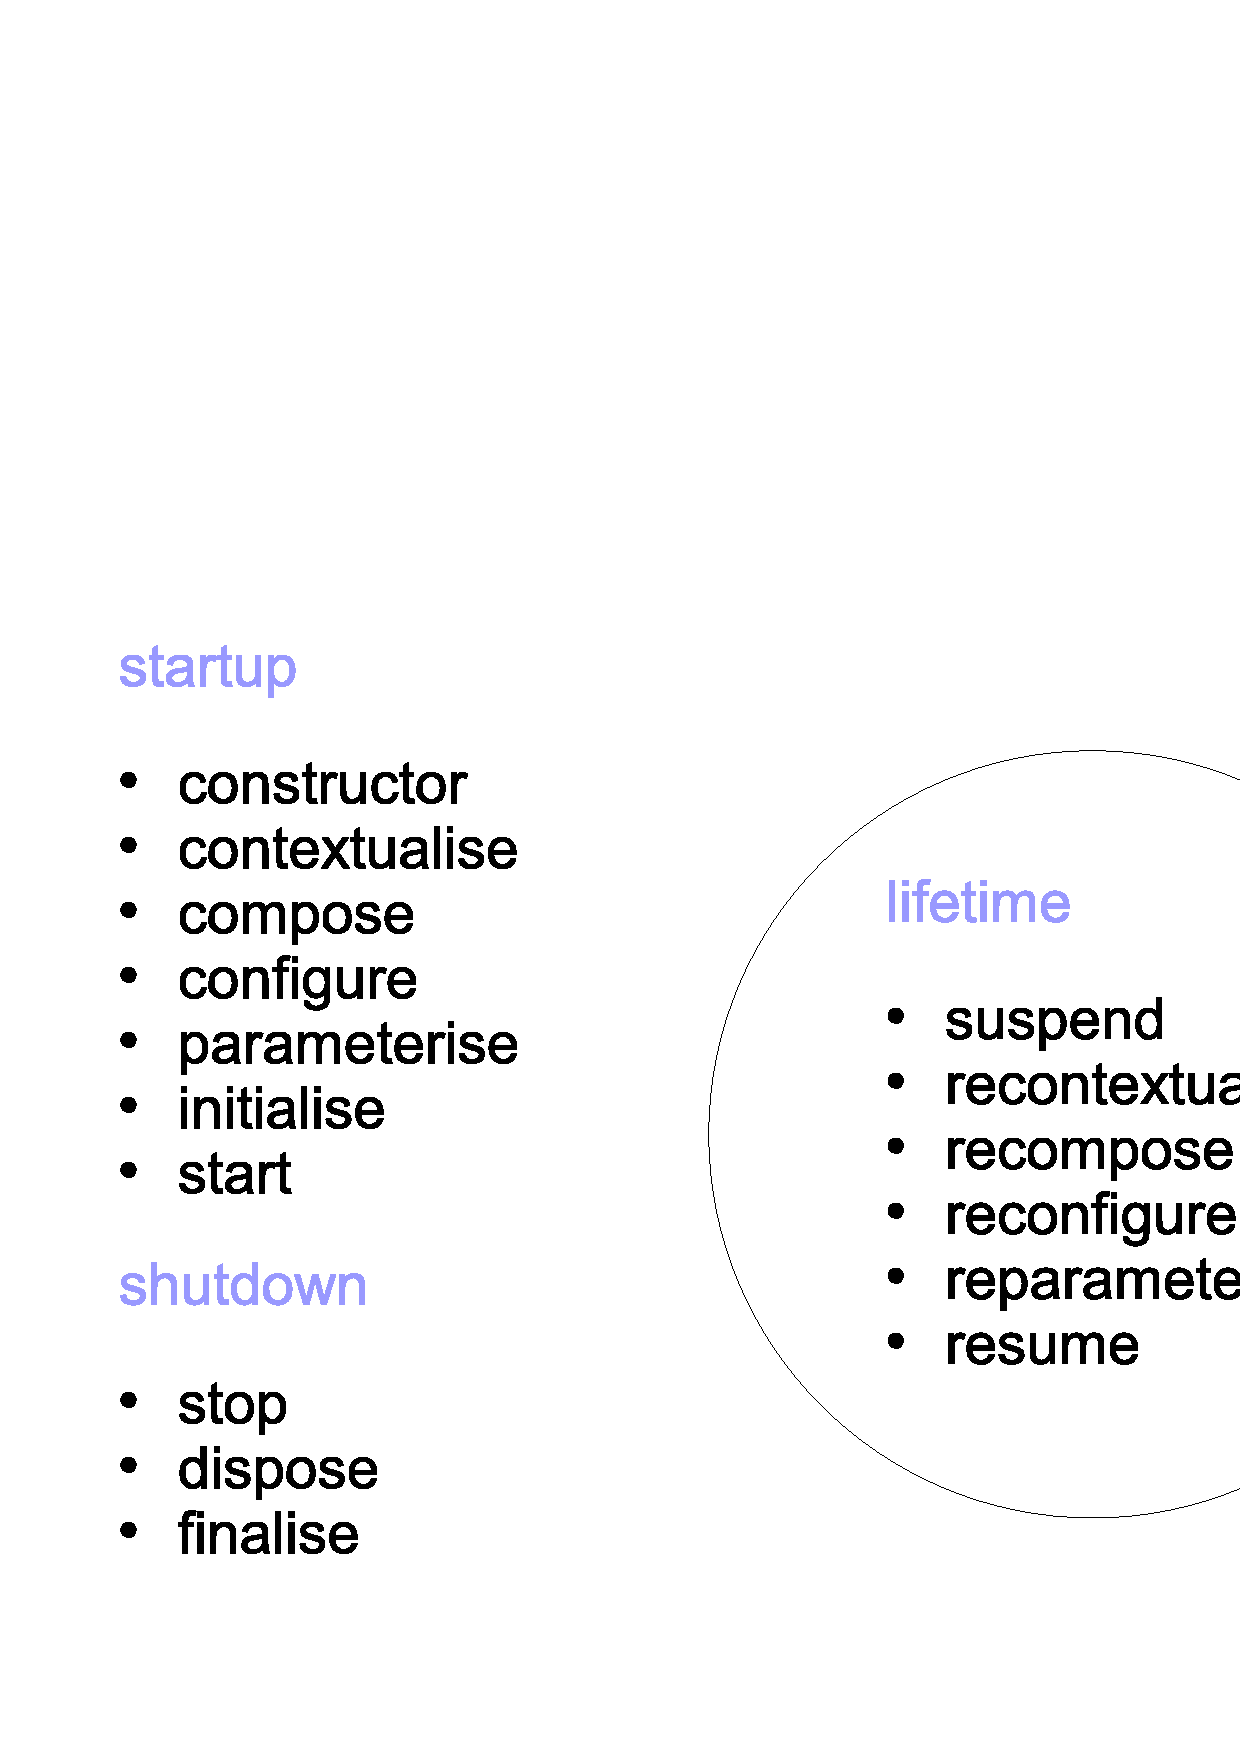
\includegraphics[scale=0.3,angle=-90]{graphic/lifecycle.pdf}
        \caption{Component Lifecycle Methods}
        \label{lifecycle_figure}
    \end{center}
\end{figure}

The lifecycle of a component specifies the methods that can be called on it,
and the order in which this may happen. The corresponding methods are called
\emph{Lifecycle Methods}. Some of them can be called only once in a specific
phase of a component's lifecycle, others may be called multiple times. The
methods in figure \ref{lifecycle_figure} are examples taken from the
\emph{Avalon} \cite{avalon} project. They represent three phases in a
component's lifecycle: \emph{Startup}, \emph{Lifetime} and \emph{Shutdown}.

Lifetime phase methods can be called repeatedly, at various times after startup
and before shutdown. The \emph{constructor} is called as a consequence of
instantiation. Its counterpart \emph{destructor} is not considered in the
project; since \emph{Avalon} is a Java-based framework, it was omitted because a
\emph{Garbage Collector} destroys instances at some indeterminate moment.

\textit{The order in which the various lifecycle methods are called is very
specific. While none are required (it is possible to have a component
implementing none of the lifecycle methods, although the use of that would be
limited), some can only be used when others are as well. It is up to each
container to indicate which lifecycle methods it will honour}, as \cite{avalon}
writes. This should be clearly documented together with the description of the
container.

A component lifecycle allows to forward parameters throughout a whole framework,
which makes static objects such as the singleton managers criticised in section
\ref{global_access_heading} superfluous. The \emph{configure} method, for
example, may forward a \emph{Configuration} object containing parameters that
otherwise would have to be made global.

%
% $RCSfile: interface_and_implementation.tex,v $
%
% Copyright (C) 2002-2008. Christian Heller.
%
% Permission is granted to copy, distribute and/or modify this document
% under the terms of the GNU Free Documentation License, Version 1.1 or
% any later version published by the Free Software Foundation; with no
% Invariant Sections, with no Front-Cover Texts and with no Back-Cover
% Texts. A copy of the license is included in the section entitled
% "GNU Free Documentation License".
%
% http://www.cybop.net
% - Cybernetics Oriented Programming -
%
% http://www.resmedicinae.org
% - Information in Medicine -
%
% Version: $Revision: 1.1 $ $Date: 2008-08-19 20:41:07 $ $Author: christian $
% Authors: Christian Heller <christian.heller@tuxtax.de>
%

\subsection{Interface and Implementation}
\label{interface_and_implementation_heading}
\index{Separation of Interface and Implementation}
\index{Java}
\index{Interface}
\index{Interface Pattern}
\index{Class}
\index{Decoupling of Components}
\index{Java Development Kit}
\index{JDK}

The \emph{Separation of Interface and Implementation} is a core concept of many
programming languages. \emph{Java}, for example, distinguishes \emph{Interface}
and \emph{Class} (section \ref{classification_heading}). Mark Grand's book
\emph{Patterns in Java} \cite{grand} refers to that separation simply as
\emph{Interface} pattern, one of whose uses, after him, were to
\emph{encapsulate components}, that is to:

\begin{itemize}
    \item[-] Force decoupling of different components
    \item[-] Ensure easy changes of interface implementations
    \item[-] Enable users to read interface documentations without having the
        implementation details clutter up their perception
    \item[-] Increase the reuse possibility in larger applications
\end{itemize}

The Java source code example below shows how the \emph{sayHello} method whose
header is declared in the \emph{HelloWorld} interface can be used as
\emph{Application Programming Interface} (API) without knowing anything about
the underlying implementation. Depending on the instance, the method may be
processed on a local or a remote system.

\begin{scriptsize}
    \begin{verbatim}
    package helloworld;
    public interface HelloWorld {
        void sayHello(String greeting);
    }

    package helloworld.impl.default;
    public class DefaultHelloWorld implements HelloWorld {
        void sayHello(String greeting) {
            System.out.println("HelloWorld Greeting: " + greeting);
        }
    }

    package helloworld.impl.remote;
    public class RemoteHelloWorld implements HelloWorld {
        private RemoteMessager remoteMessager;
        public RemoteHelloWorld(RemoteMessager rm) {
            remoteMessager = rm;
        }
        void sayHello(String greeting) {
            rm.sendMessage("HelloWorld Greeting: " + greeting);
        }
    }
    \end{verbatim}
\end{scriptsize}

Further details and recommendations for using interfaces, on examples specific
to the \emph{Java Development Kit} (JDK) \cite{java}, are given in \cite{avalon}.

%
% $RCSfile: separation_of_concerns.tex,v $
%
% Copyright (C) 2002-2008. Christian Heller.
%
% Permission is granted to copy, distribute and/or modify this document
% under the terms of the GNU Free Documentation License, Version 1.1 or
% any later version published by the Free Software Foundation; with no
% Invariant Sections, with no Front-Cover Texts and with no Back-Cover
% Texts. A copy of the license is included in the section entitled
% "GNU Free Documentation License".
%
% http://www.cybop.net
% - Cybernetics Oriented Programming -
%
% http://www.resmedicinae.org
% - Information in Medicine -
%
% Version: $Revision: 1.1 $ $Date: 2008-08-19 20:41:08 $ $Author: christian $
% Authors: Christian Heller <christian.heller@tuxtax.de>
%

\subsection{Separation of Concerns}
\label{separation_of_concerns_heading}
\index{Separation of Concerns}
\index{SoC}
\index{Container}
\index{Component}
\index{Contract}
\index{Separation of Contract and Implementation}
\index{Concern}
\index{Component Oriented Programming}
\index{COP}
\index{Role of a Component}
\index{Electronic Health Record}
\index{EHR}
\index{Service Manager for Components}
\index{Lookup Method identifying Components}
\index{Fully Qualified Name}
\index{FQN}
\index{Component Selector}

The \emph{Avalon} project \cite{avalon} writes:

\begin{quote}
    Separation of concerns in its simplest form is separating a problem into
    different points of view. Every time one uses interfaces within object- or
    component oriented programming, the \emph{Separation of Concerns} (SoC)
    pattern is applied. The interface separates the implementation concern from
    the concern of the user of the interface.
\end{quote}

Interfaces \emph{pool} common methods (section \ref{classification_heading}).
Inheriting an interface, components indicate to their surrounding container
which methods they implement so that the container can use and rely on these.
Therefore, one often talks of a \emph{Contract} between container and
component. The contract defines what the container (as user of the component)
must provide and what the component produces. In the end, the separation of
\emph{Interface and Implementation} (section
\ref{interface_and_implementation_heading}) could be more correctly called
separation of \emph{Contract and Implementation}.

The contract was mentioned in section \ref{component_lifecycle_heading} which
explained that a container is responsible for taking its components through a
lifecycle. The \emph{Avalon} project \cite{avalon} specifies a number of
concerns which enforce the implementation of one or more lifecycle methods.
Here is a list of some concerns referring to the methods of section
\ref{component_lifecycle_heading}:

\begin{itemize}
    \item[-] Loggable
    \item[-] Contextualizable
    \item[-] Composable
    \item[-] Configurable
    \item[-] Initializable
    \item[-] Startable
    \item[-] Suspendable
\end{itemize}

For example, an object that can be configured implements the \emph{Configurable}
interface. The contract surrounding that interface is that the container as
instantiator of the object passes a \emph{Configuration} object to the component
being a configurable object. Just what the configurable object does with the
passed configuration object is irrelevant to the instantiator.

\begin{figure}[ht]
    \begin{center}
        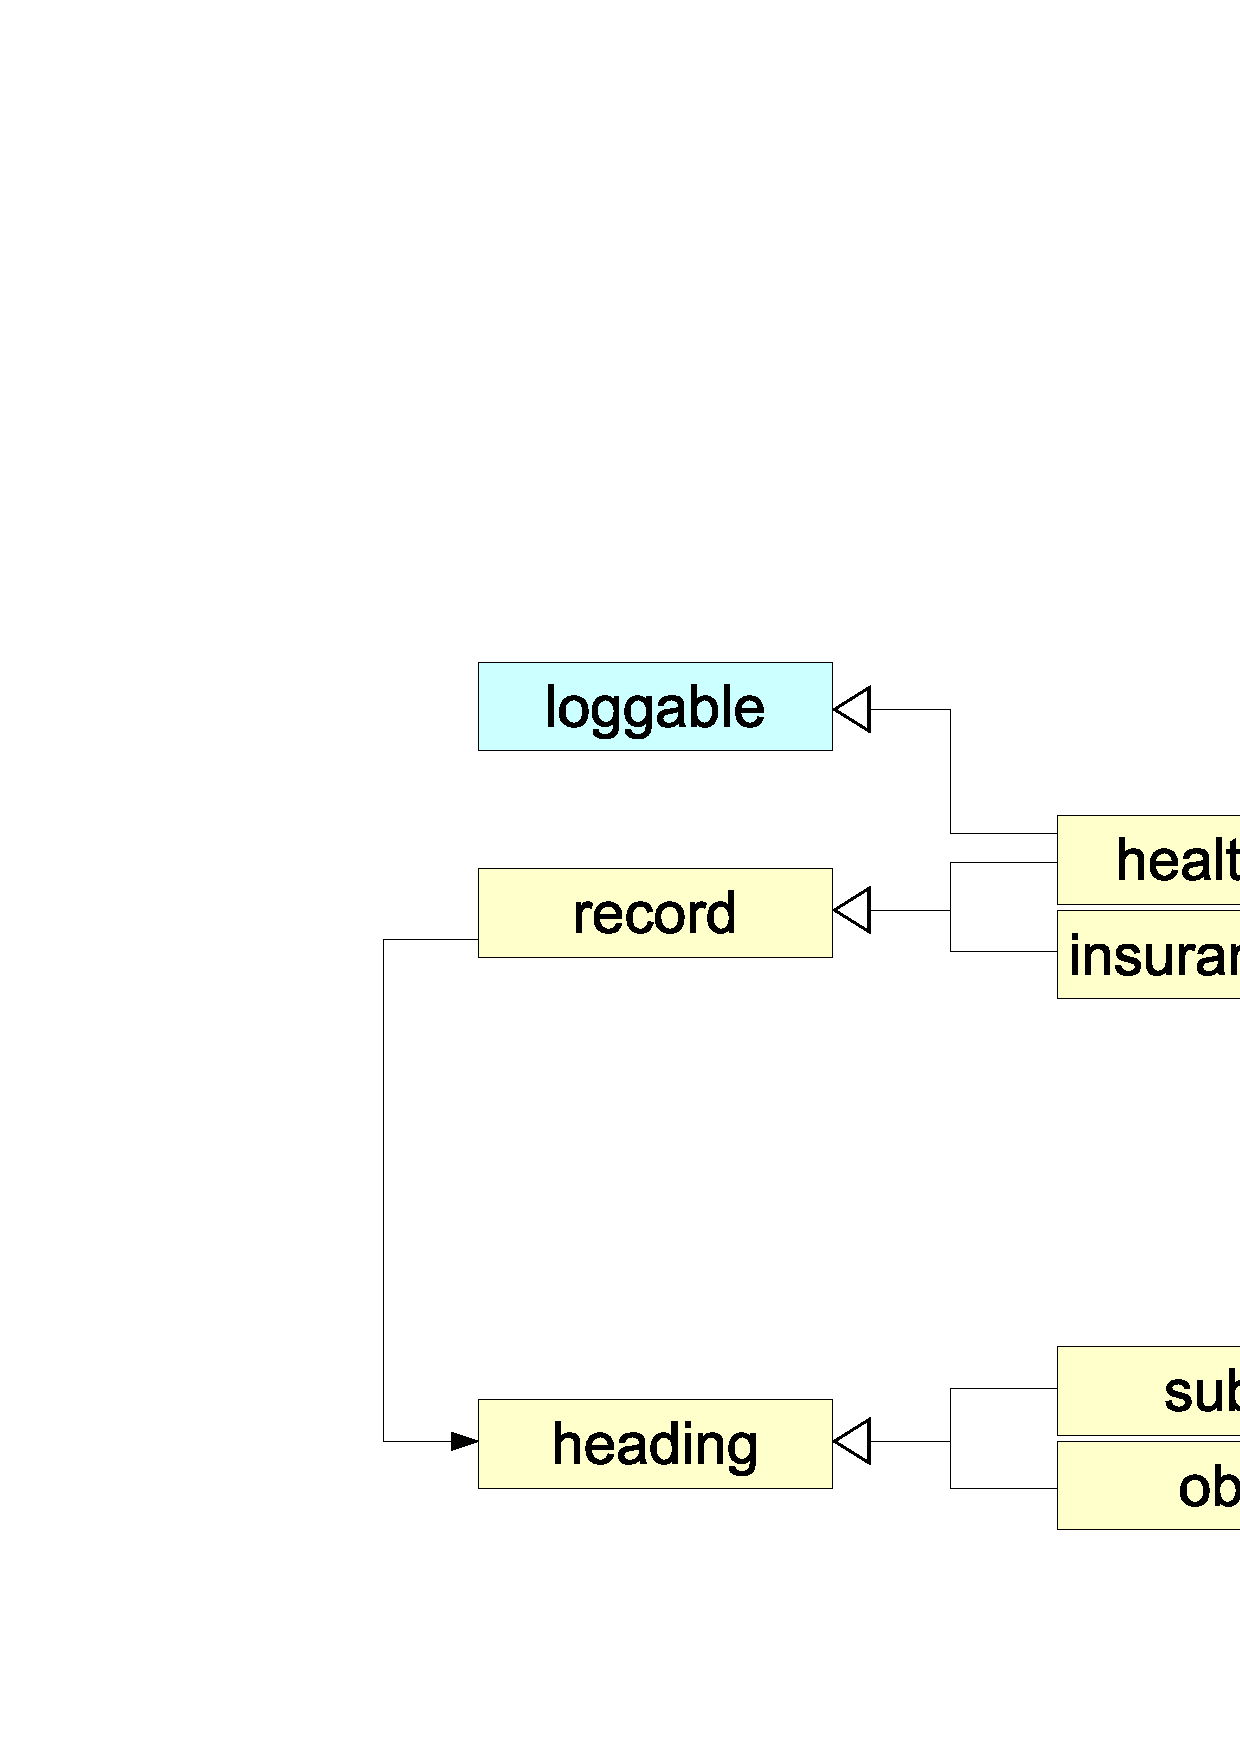
\includegraphics[scale=0.3,angle=-90]{graphic/concern.pdf}
        \caption{Class Inheriting Loggable Concern Interface}
        \label{concern_figure}
    \end{center}
\end{figure}

Figure \ref{concern_figure} shows an \emph{Electronic Health Record} (EHR)
component implementing the \emph{Loggable} interface which indicates that the
component offers functionality for the logging of messages. To fully explain
the figure: The EHR inherits from a general \emph{Record} class that references
so-called \emph{Heading} objects which may be a \emph{Subjective} description
of a patient or an \emph{Objective} result of an examination. Of course, these
objects may be programmed as components as well.

A common comparison used in component oriented programming is that of the
\emph{Role} coming from theater \cite{avalon}. The function or action of a
component's role within a system, as well as its contracts, are defined by its
script -- the interface. Any object that implements the component interface
must comply with the contracts. This allows developers to manipulate components
using a standard interface, without worrying about the semantics of the
implementation. They are separate concerns.

A \emph{Service Manager} is often used to get an instance of the needed
component. The manager's \emph{lookup} method identifies the component based on
the \emph{Fully Qualified Name} (FQN) of the role (interface). If several
components functioning in the same role exist, a \emph{Component Selector} may
be applied to choose the right one. More details are given in \cite{avalon}.

%
% $RCSfile: spread_functionality.tex,v $
%
% Copyright (C) 2002-2008. Christian Heller.
%
% Permission is granted to copy, distribute and/or modify this document
% under the terms of the GNU Free Documentation License, Version 1.1 or
% any later version published by the Free Software Foundation; with no
% Invariant Sections, with no Front-Cover Texts and with no Back-Cover
% Texts. A copy of the license is included in the section entitled
% "GNU Free Documentation License".
%
% http://www.cybop.net
% - Cybernetics Oriented Programming -
%
% http://www.resmedicinae.org
% - Information in Medicine -
%
% Version: $Revision: 1.1 $ $Date: 2008-08-19 20:41:09 $ $Author: christian $
% Authors: Christian Heller <christian.heller@tuxtax.de>
%

\subsection{Spread Functionality}
\label{spread_functionality_heading}
\index{Spread Functionality}
\index{Redundant Code}
\index{Overlapping Code through Concerns}
\index{Spread Functionality through Concerns}
\index{Layer Supertype Pattern}
\index{Lifecycle Method}
\index{Concern-less Development}
\index{Class Hierarchy}
\index{Ontology}

\begin{figure}[ht]
    \begin{center}
        \includegraphics[scale=0.3,angle=-90]{graphic/redundant.pdf}
        \caption{Redundant Code through Usage of Concerns}
        \label{redundant_figure}
    \end{center}
\end{figure}

Separating concerns does not avoid \emph{Redundant Code}. If two independent
components want to target the same concern what they expose by implementing the
corresponding interface, they will both have to implement the required methods
redundantly. This may not be a problem with just two records as in the example
of figure \ref{redundant_figure}, but will become an issue as soon as other
objects are to be programmed as component as well.

Another unwanted effect when using concern interfaces is the \emph{Overlapping}
of concerns (figure \ref{overlapping_figure}). It may happen that a superclass
implements a number of lifecycle methods and their corresponding interfaces
without knowing if its subclasses eventually implement exactly one of these,
too. In such a case, redundant code would appear and the principle of efficient
programming would be injured once more.

\begin{figure}[ht]
    \begin{center}
        \includegraphics[scale=0.3,angle=-90]{graphic/overlapping.pdf}
        \caption{Overlapping Code through Usage of Concerns}
        \label{overlapping_figure}
    \end{center}
\end{figure}

A piece of source code holding a reference to a component instance in form of
a concern interface can \emph{only} call the methods of \emph{that} concern.
Mostly, however, other methods have to be called as well. In this case, a
\emph{Downcast} from the concern interface to the component class implementing
the interface becomes necessary. Yet to be able to downcast, the class (type)
to downcast to needs to be known anyway. In the end, the usability of concern
interfaces turns out to be limited, sometimes even useless, since they only
allow a few methods to be called and information about the real class is not
available.

\begin{figure}[ht]
    \begin{center}
        \includegraphics[scale=0.3,angle=-90]{graphic/spreadbunch.pdf}
        \caption{Concerns Spread Functionality, an Ontology Bunches it}
        \label{spreadbunch_figure}
    \end{center}
\end{figure}

From the viewpoint of reuse, it seems far better to inherit all components from
one common super-class, as suggested by the \emph{Layer Supertype} pattern
(section \ref{layer_supertype_heading}). This class would implement necessary
lifecycle methods just once, being available for all inheriting classes. For the
used example this would mean to eliminate all \emph{Loggable} concern interfaces
(figure \ref{spreadbunch_figure}) and put the logging functionality into the
\emph{Record} super class.

Finally, the only way out of the misery of redundant code caused by concern
interfaces seems to be \emph{Concern-less} software development using
\emph{pure} class hierarchies. And in fact, this is what \emph{Ontologies}
(section \ref{ontology_heading}) are proposing. Section
\ref{separation_of_concerns_heading} mentioned that interfaces help
\emph{pooling} common methods; but in the big system picture, they actually
\emph{spread} them. While concerns represented by interfaces \emph{spread}
functionality, away from the classes that were actually made to \emph{keep} it,
an ontology \emph{bunches} functionality. Chapter \ref{knowledge_schema_heading}
will show some ontology examples and introduce a knowledge schema for their
hierarchical representation, including necessary meta information.

%
% $RCSfile: aspect_oriented_programming.tex,v $
%
% Copyright (C) 2002-2008. Christian Heller.
%
% Permission is granted to copy, distribute and/or modify this document
% under the terms of the GNU Free Documentation License, Version 1.1 or
% any later version published by the Free Software Foundation; with no
% Invariant Sections, with no Front-Cover Texts and with no Back-Cover
% Texts. A copy of the license is included in the section entitled
% "GNU Free Documentation License".
%
% http://www.cybop.net
% - Cybernetics Oriented Programming -
%
% http://www.resmedicinae.org
% - Information in Medicine -
%
% Version: $Revision: 1.1 $ $Date: 2008-08-19 20:41:05 $ $Author: christian $
% Authors: Christian Heller <christian.heller@tuxtax.de>
%

\subsection{Aspect Oriented Programming}
\label{aspect_oriented_programming_heading}
\index{Aspect Oriented Programming}
\index{AOP}
\index{Object Oriented Programming}
\index{OOP}
\index{Concern Interface}
\index{Aspect}
\index{Meta Object Protocol}
\index{MOP}
\index{Mixin Programming Concept}
\index{Crosscutting Concern}
\index{Common Concern}
\index{Aspect Marker Interface}
\index{Component Oriented Programming}
\index{COP}
\index{Development Aspect}
\index{Production Aspect}
\index{Join Point}
\index{Pointcut}
\index{Advice}
\index{Inter-Type Declaration}
\index{Aspect Oriented Software Development}
\index{AOSD}
\index{Aspect Weaver}
\index{Join Point Representation}
\index{Join Point Model}
\index{JPM}
\index{Singleton Pattern}
\index{Lifecycle Method}

Another alternative avoiding redundant code caused by the implementation of
concern interfaces (section \ref{separation_of_concerns_heading}) is the
so-called \emph{Aspect Oriented Programming} (AOP), which is an extension to
\emph{Object Oriented Programming} (OOP). \emph{Aspects} are a possibility to
separate and define concern areas addressed in program code. Wikipedia
\cite{wikipedia} writes that:

\begin{quote}
    Aspects emerged out of object-oriented programming and have functionality
    similar to using a meta-object protocol (section \ref{reflection_heading}).
    Aspects relate closely to programming concepts like subjects, mixins, and
    delegation.
\end{quote}

The Avalon documentation \cite{avalon} means that AOP were: \textit{the next
logical step after separation of concerns}. Many concerns could not be
centrally addressed using the standard mechanisms of programming. Using AOP, it
were possible to do so in a simple fashion.

The AspectJ documentation \cite{aspectj} writes that the motivation for AOP had
been the realisation that there are issues or concerns (like a security policy)
that cut across many of the natural units of modularity of an application and
are not well captured by traditional programming methodologies. For
\emph{Object Oriented Programming} (OOP) languages, the natural unit of
modularity were the \emph{Class}. But in these languages, some concerns were
not easily turned into classes because they'd \emph{cut across} classes. So
these weren't reusable, couldn't be refined or inherited, were spread
throughout the program in an undisciplined way and, in short, were difficult to
work with. AOP were a way of modularising \emph{Crosscutting Concerns} much
like OOP were a way of modularising \emph{Common Concerns}. The later chapter
\ref{statics_and_dynamics_heading} will come back to these two kinds of
concerns in short.

As shown in the previous sections, the \emph{Avalon} project \cite{avalon} uses
concern interfaces (sometimes called \emph{Aspect Marker Interfaces}) and
\emph{Component Oriented Programming} (COP) to define its concerns, what
frequently leads to redundant implementations. Other projects, for instance
\emph{AspectJ} \cite{aspectj} and \emph{AspectWerkz} \cite{aspectwerkz},
provide AOP facilities whose aim is the clean modularisation of crosscutting
concerns such as those in the following list, which AspectJ divides into
\emph{Development Aspects}:

\begin{itemize}
    \item[-] Tracing
    \item[-] Profiling and Logging
    \item[-] Pre- and Post-Conditions
    \item[-] Contract Enforcement
    \item[-] Configuration Management
\end{itemize}

and \emph{Production Aspects}:

\begin{itemize}
    \item[-] Change Monitoring
    \item[-] Context Passing
    \item[-] Providing Consistent Behaviour
\end{itemize}

The AspectJ project as an implementation of AOP for Java adds just one new
concept to that language -- the \emph{Join Point}, which is a well-defined
point in the program flow. A number of new constructs are introduced as well: A
\emph{Pointcut} picks out certain join points and values at those points; an
\emph{Advice} is a piece of code that is executed when a join point is reached.
Both do dynamically affect the program flow. \emph{Inter-Type Declarations}, on
the other hand, statically affect a program's class hierarchy, namely the
members of its classes and the relationships between classes. AspectJ's
\emph{Aspect}, finally, is the unit of modularity for crosscutting concerns. It
behaves somewhat like a Java class, summarising the constructs described
before, that is pointcuts, advices and inter-type declarations.

\emph{Aspect Oriented Software Development} (AOSD) is about developing programs
that rely on AOP principles and languages -- or language extensions,
respectively. Such programs get compiled slightly differently than usual. An
\emph{Aspect Weaver} generates a \emph{Join Point Representation} of the
program, by merging code and aspects. Only afterwards, the program is compiled
into an executable.

Although AOP seems to successfully address the problem of crosscutting concerns,
it also brings with yet another programming paradigm that application developers
have to get familiar with. The new concepts and constructs further complicate
software development. The source code gets further fractured because of AOP's
additional modules. It is harder to follow the program flow and one has less
control on the behaviour of classes, so that the usage of development tools
becomes inevitable. But besides this rather general criticism, there is more
specific ones: The \emph{Join Point Model} (JPM), for example, is reviewed in
\cite{huttenhuis} which points out some unsolved issues in AOP, while
investigating the following properties of join points:

\begin{itemize}
    \item[-] \emph{Granularity:} only some locations in program code are
        suitable as join points
    \item[-] \emph{Encapsulation:} there is no effective way to protect join
        points from aspect-imposed modification
    \item[-] \emph{Semantics:} low-level join point identification leads to
        tight coupling between aspects and join points
    \item[-] \emph{Jumping Aspects:} context-sensitive join points execute
        different aspect code
    \item[-] \emph{Sharing:} dependencies and order of execution are unclear
        when having several pieces of advice at the same join point
\end{itemize}

At least some of the concerns that AOP addresses could be implemented with
lifecycle-techniques as well. A logger, for example, could be created once at
system startup. But instead of accessing it across static methods, as suggested
by the \emph{Singleton} pattern (section \ref{singleton_heading}), or executing
an aspect-oriented \emph{Advice} when a join point is reached, the reference to
the logger instance could simply be forwarded from component to component,
using a special \emph{globalise} lifecycle method, so that each would be able
to access the logger. However, also this solution becomes tedious with a
growing number of objects to be forwarded. The new kind of programming
introduced in part \ref{contribution_heading} of this work therefore suggests
to put general functionality (concerns, aspects) into an interpreter program
acting close to hardware and providing the general functionality to application
systems executed by it.

%
% $RCSfile: agent_oriented_programming.tex,v $
%
% Copyright (C) 2002-2008. Christian Heller.
%
% Permission is granted to copy, distribute and/or modify this document
% under the terms of the GNU Free Documentation License, Version 1.1 or
% any later version published by the Free Software Foundation; with no
% Invariant Sections, with no Front-Cover Texts and with no Back-Cover
% Texts. A copy of the license is included in the section entitled
% "GNU Free Documentation License".
%
% http://www.cybop.net
% - Cybernetics Oriented Programming -
%
% http://www.resmedicinae.org
% - Information in Medicine -
%
% Version: $Revision: 1.1 $ $Date: 2008-08-19 20:41:05 $ $Author: christian $
% Authors: Christian Heller <christian.heller@tuxtax.de>
%

\subsection{Agent Oriented Programming}
\label{agent_oriented_programming_heading}
\index{Agent Oriented Programming}
\index{AGOP}
\index{Component Oriented Programming}
\index{COP}
\index{Inversion of Control Pattern}
\index{IoC}
\index{Application Programming Interface}
\index{API}
\index{Active Component}
\index{Passive Component}
\index{Agent}
\index{Multi Agent System}
\index{MAS}
\index{Agent Communication Language}
\index{ACL}
\index{Language Paradigm}
\index{Ontology}
\index{Mobility of an Agent}
\index{Object Oriented Programming}
\index{OOP}
\index{Speech Act Theory}
\index{Belief of an Agent}
\index{Capability of an Agent}
\index{Decision of an Agent}
\index{Mental State of an Agent}
\index{Knowledge Base of an Agent}
\index{Agent0 Language}

Components created after the principles of \emph{Component Oriented Programming}
(COP) are \emph{passive}, because they follow the \emph{Inversion of Control}
(IoC) pattern. The functionality, or \emph{Service}, they offer is called by a
surrounding container, via a well-defined \emph{Application Programming Interface}
(API). \emph{Active} components, on the other hand, act alone. An \emph{Agent}
is a self-acting component. It runs \emph{autonomically} or
\emph{semi-autonomically}, is \emph{proactive}, \emph{reactive} and
\emph{social} \cite[p. 330]{sowa}. Many individual communicative software
agents may form a \emph{Multi Agent System} (MAS) \cite{wikipedia}.
Communication happens by some \emph{Agent Communication Language} (ACL)
(section \ref{agent_communication_language_heading}). David Parks, who calls
\emph{Agent Oriented Programming} (AGOP) a \emph{Language Paradigm}, writes
\cite{parks}:

\begin{quote}
    In AGOP, objects known as agents interact to achieve individual goals.
    Agents can exist in a structure as complex as a global internet or one as
    simple as a module of a common program. Agents can be autonomous entities,
    deciding their next step without the interference of a user, or they can be
    controllable, serving as a mediary between the user and another agent.
\end{quote}

In search for a uniform definition of the term \emph{Agent}, Ralf Kuehnel
investigated numerous sources of literature but finally comes to the conclusion
\cite[p. 203]{kuehnel} that the term is just a \emph{Metaphor} standing for
different properties, depending on the field it is used in. Typically mentioned
means of agents, however, are \cite[p. 11]{kuehnel}: \emph{Distribution}, common
\emph{Language} and \emph{Ontology} (section \ref{conceptual_network_heading}),
\emph{Cooperation} and \emph{Coordination}, \emph{Security} and \emph{Mobility}.

Comparing \emph{Agents} of AGOP with \emph{Objects} known from OOP, Parks
\cite{parks} writes: \textit{It is not clear, for example, what the concepts of
inheritance and dynamic dispatch mean when discussing an agent.} He points out
the following significant differences:

\begin{itemize}
    \item[-] The fields of an agent are restricted. The state of an agent is
        described in terms of \emph{Beliefs}, \emph{Capabilities} and
        \emph{Decisions} (\emph{Obligation} / \emph{Commitment}). These ideas
        are built into the syntax of the language.
    \item[-] Each message is also defined in terms of mental activities. An agent
        may engage another (or itself) with messaging activities from a restricted
        class of categories. In Shoham's formalism \cite{shoham}, the categories
        of messages are taken from \emph{Speech-Act Theory}; they are:
        \emph{Informing}, \emph{Requesting}, \emph{Offering}, \emph{Accepting},
        \emph{Rejecting}, \emph{Competing} and \emph{Assisting}.
\end{itemize}

Yoav Shoham, who presented AGOP as a new way to describe intelligent agents
\cite{shoham}, suggests that an AGOP system needs three elements to be
complete, a:

\begin{enumerate}
    \item[-] \emph{Formal Language} with clear syntax for describing the mental state
    \item[-] \emph{Programming Language} in which to define agents
    \item[-] \emph{Method} for converting neutral applications into agents
\end{enumerate}

To the \emph{Mental State} of an agent belong information \cite{kuehnel} about its:

\begin{itemize}
    \item[-] \emph{Environment} (constraints)
    \item[-] \emph{Expertise} (capabilities) and \emph{Motivations} (aims)
    \item[-] \emph{Actions} and \emph{Plans}
\end{itemize}

Tim Finin et al. \cite{kqml} classify the statements in a knowledge base into
two categories: \emph{Beliefs} and \emph{Goals}. After them, an agent's beliefs
encoded information it has about itself (capabilities) and its external
environment (constraints), including the knowledge bases of other agents. An
agent's goals encoded states of its external environment that the agent would
act to achieve.

To a running \emph{Agent} system belong the following modules \cite{kuehnel}:

\begin{itemize}
    \item[-] \emph{Knowledge Base:} mental state, as described above
    \item[-] \emph{Controller:} task controller, scheduler and option selection algorithm
    \item[-] \emph{Executor:} task runner and security
    \item[-] \emph{Interaction:} communication handler, sender and receiver
    \item[-] \emph{Management:} lifecycle manager, startup and shutdown
\end{itemize}

While early research in AGOP used special languages like Shoham's \emph{Agent0}
\cite{shoham}, agent-oriented systems created later were also built upon OOP-
and other contemporary programming paradigms \cite[p. 237]{kuehnel}. Ralf
Kuehnel \cite{kuehnel} calls \emph{Agent0} alone a \textit{very limited
programming language} and takes this as evidence for supporting both, the
development of agents and the representation of knowledge with a framework based
on OOP principles. For the implementation of this framework, his choice fell on
Java as system programming language (section \ref{system_programming_heading}).

That is, although AGOP suggests the separation of a system's \emph{Knowledge}
(mental state) from its internal runtime processing and \emph{Control} (agent)
and sees them both as separate elements that should be implemented in
\emph{different} languages (\emph{formal} vs. \emph{programming}), as mentioned
by Shoham (see above), many agent-oriented systems use just \emph{one} language
for implementing both. Even if they are kept in different modules, the conceptual
differences between \emph{high-level} application knowledge and \emph{low-level}
system control cannot be honoured sufficiently. This \emph{Mix-up} puts them on
the same level like traditional systems. \emph{Cybernetics Oriented Programming}
(CYBOP) as described in this work therefore defines a knowledge modelling
language (chapter \ref{cybernetics_oriented_language_heading}) which is
independent from the implementation language of its underlying interpreter.

Furthermore, if OO concepts like \emph{Composition} or \emph{Inheritance} were
present in knowledge models, the usage of an OOP language to implement the actual
agent system could \emph{not} be justified any longer. In such a case, lower-level
\emph{Structured and Procedural Programming} (SPP) languages would suffice, and
work much more efficiently. Chapter \ref{cybernetics_oriented_interpreter_heading}
of this work introduces a knowledge interpreter that is written in the \emph{C}
programming language. The interpreter owns a knowledge base keeping all
application knowledge, and it has modules for lifecycle management, signal
(event) processing, communication etc., just like the definition of an agent
(see above) suggests.

